%-------------------------------------------------------------------------------------------------------
%-------------------------------------------------------------------------------------------------------
\chapter{The LCS Runtime Library RtLib}

Intended for the node firmware programmer, the LCS runtime library is the main interface to the hardware module. The library has methods for node and port configuration, event processing and layout control bus management. Most of the LCS bus management, node, port and port data management is performed transparently to the node firmware programmer. The library also provides convenience methods to send messages to other nodes and allows for a rich set of callback functions to be registered to act on messages and events.

The key design objective for the runtime library is to relief the LCS nodes firmware programmer as much as possible from the details of running a firmware inside a hardware module. Rather than implementing the lower layers for storage and message processing at the firmware level, the runtime library will handle most of this processing transparently to the upper firmware layer. A small set of intuitive to use and easy to remember functions make up the core library. The library communicates back to the firmware layer via a set of defined callbacks. Throughout the next chapters, the library will be presented in considerable detail. Let's start with the high level view.

The following figure depicts the overall structure of a LCS hardware module and node. At the bottom is the hardware module, which contains the communication interfaces, the controller and the node specific functions. The core library offers a set of APIs and callbacks to the node firmware. The firmware programmer can perform functions such as sending a message or accessing a node attribute through the APIs provided. The library in turn communicates with the firmware solely via registered callbacks.

picture 

\begin{figure}[h]
    \centering
   % 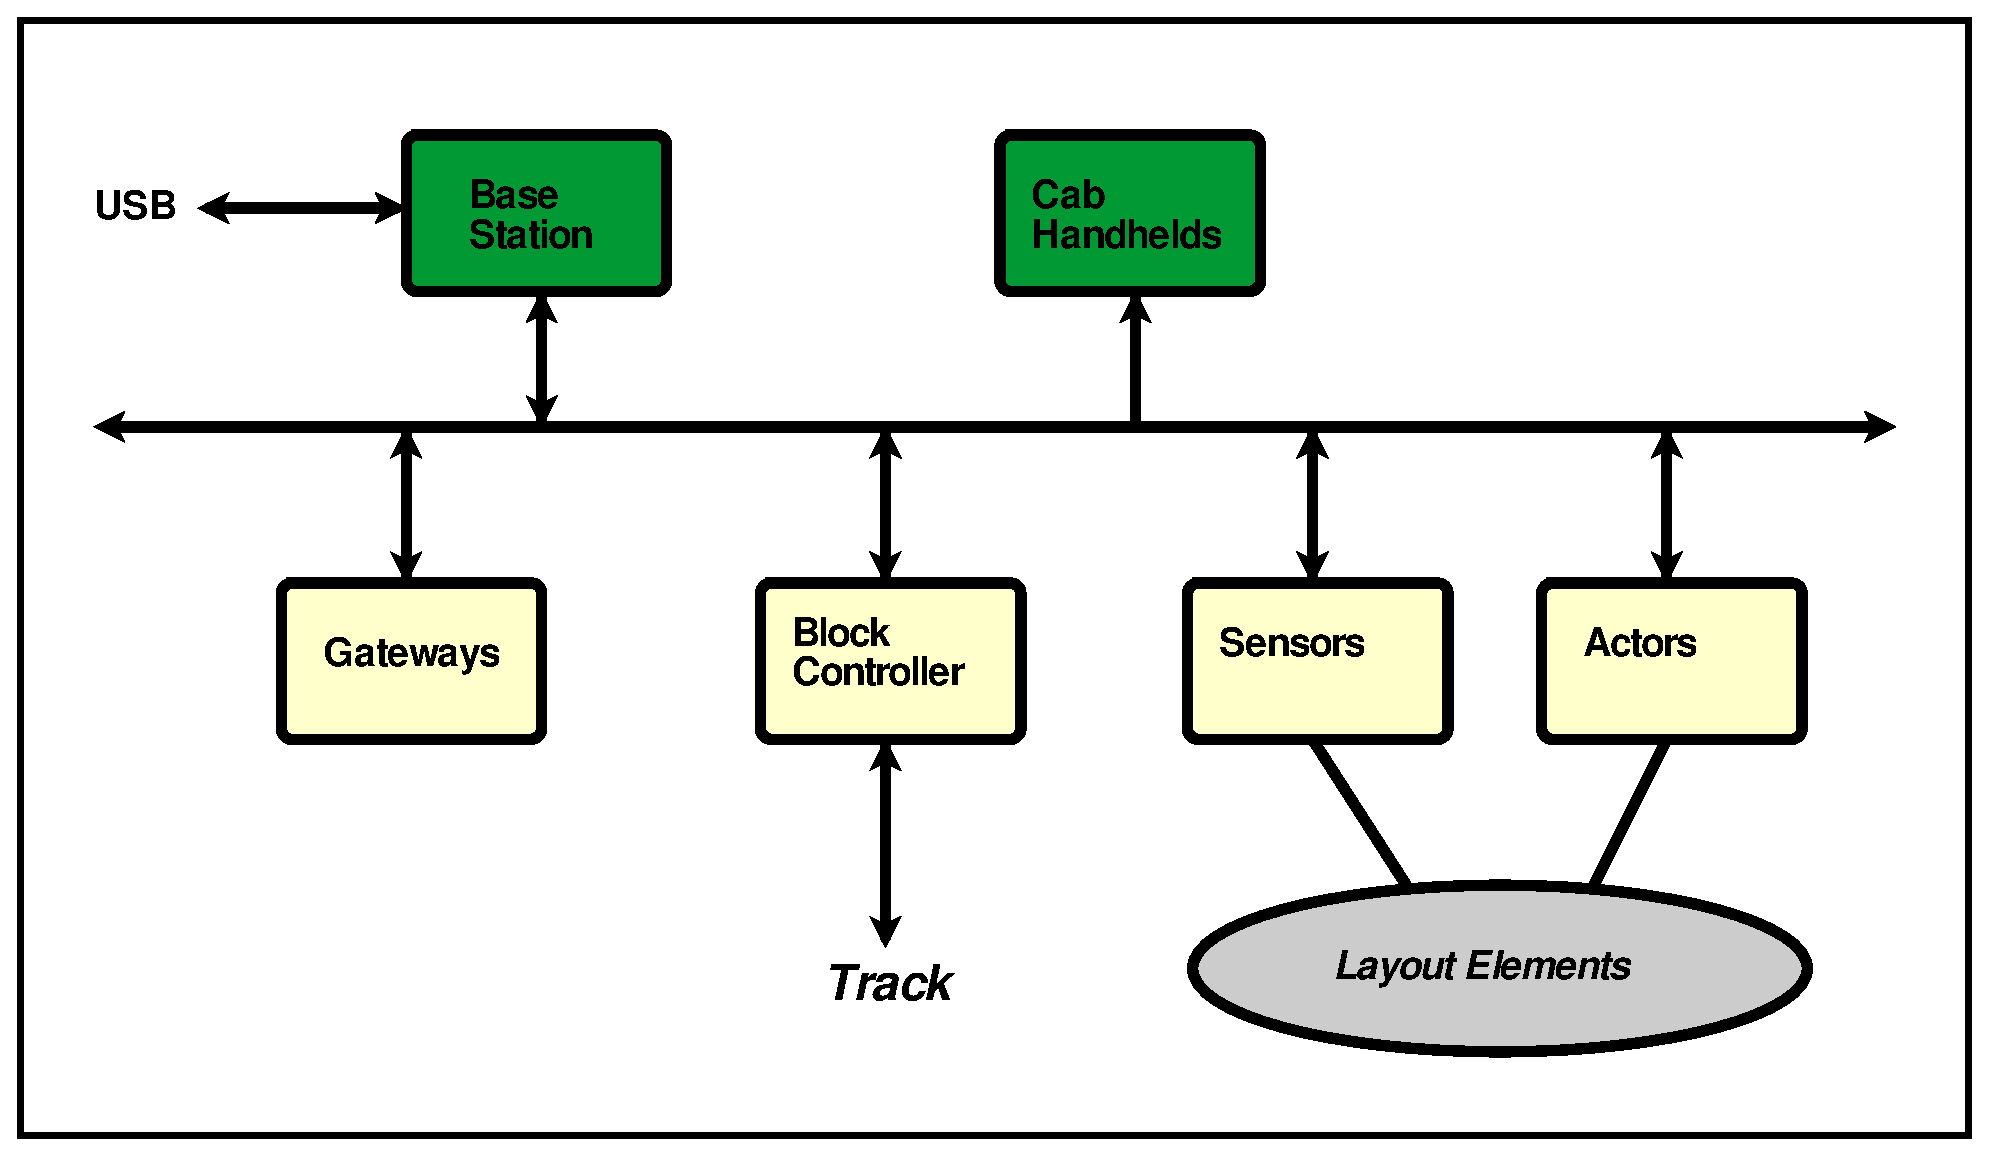
\includegraphics[page=1, width=\textwidth]{./figures/Schematic_LcsNodes-Layout-Overview.pdf}
   %![Schematic_LcsNodes-Core-Library-Overview.png](./Figures/Schematic_LcsNodes-Core-Library-Overview.png )
\end{figure}

The firmware has of course also direct access to the hardware module capabilities. This is however outside the scope for the LCS core library. As we will see in the coming chapters, the library has a rich set of functions and does also perform many actions resulting form the protocol implementation transparently to the firmware programmer. It is one of the key ideas, that the firmware programmer can concentrate on the module design and not so much on the inner workings of the LCS layout system. Events, ports, nodes and attributes form a higher level foundation for writing LCS control system firmware. Not all of the functionality will of course be used by every node. A base station and a handheld cab control will for example make heavy use of the DCC commands. A turnout device node will use much more of the port and event system. Size and functions of the various library components can be configured for a node.

As a consequence, the library is not exactly a small veneer on top of the hardware and does take its program memory toll on controller storage. However, with the growing capabilities of modern controllers, this should not be a great limitation. The first working versions required an Arduino Atmega1284 alike version as the controller. The current working version is based on the Raspberry Pi Pico controller. More on the individual requirements and selection later.

The appendix contains the detailed description of all library interfaces. If a picture says more than a thousands words, an excerpt of the data declarations from the implementation says even more to the firmware programmer. At the risk of some minor differences on what is shown in the book and the actual firmware, you will find a lot of declarations directly taken from the "LcsRuntimeLib.h" include file.
